
\documentclass{PoS}

\title{Single top production measurements at the LHC: t-channel}

\ShortTitle{Single top production measurements at the LHC: t-channel}

\author{
    \speaker{Matthias Komm}\\
    Universite Catholique de Louvain (UCL) (BE)\\
    E-mail: \email{Matthias.Komm@cern.ch}
}

\abstract{
At the LHC, single top quark are predominately produced via the $t$-channel. Measuring the properties of the production process provides a vital probe of the theory of electroweak interactions. This note reviews recent results on cross section measurements and coupling structure studies in pp collisions by the ATLAS and CMS collaborations at center-of-mass energy of 7, 8, and 13~TeV.
}

\FullConference{
    8th International Workshop on Top Quark Physics\\
    14-18 September, 2015\\
    Ischia, Italy
}

\begin{document}

\section{Introduction}
The production and decay of single top quarks via $t$-channel soley involves electroweak interactions at leading order (LO). The high mass of the top quark allows it to decay to on-shell W bosons before hadroniztation becomes relevant. This allows to measure a variety of standard model (SM) properties such as the CKM matrix element $\mathrm{V_{tb}}$ and the parity-violating V-A coupling structure by studying this process. Furthermore, the top quark may be relevant in beyond-SM theories because it has the highest coupling strength to the Higgs boson and thus contributes to the Higgs self-energy and vaccum stability.

In the following, the latest results by the ATLAS and CMS collaborations are reviewed.

\section{Cross section measurements at 8~TeV}
Precise measurements of the $t$-channel single top cross section at 8~TeV have been accomplished at the LHC in pp collisions by the ATLAS and CMS collaborations~\cite{atlas-xsec8,cms-xsec8,CMS-PAS-TOP-15-007} utilizing data that corresponds to approximately $20~\mathrm{fb}^{-1}$. For the measurements, events with an isolated muon or electron and two jets are selected where one jet is required to pass the threshold of a dedicated b-tagging algorithm. The cross section is measured through a maximum likelihood fit to a discriminating variable. CMS exploits the pseudo rapidity distribution of the non b-tagged jet that is produced in the forward detector region for single top events (Fig.~\ref{fig:fit-xsec-8}a) whereas ATLAS combines multiple observables in one powerful discriminant by training a neutral network (Fig.~\ref{fig:fit-xsec-8}b).

\begin{figure}[htbp]
\begin{center}
\parbox[t]{0.5\textwidth}{\centering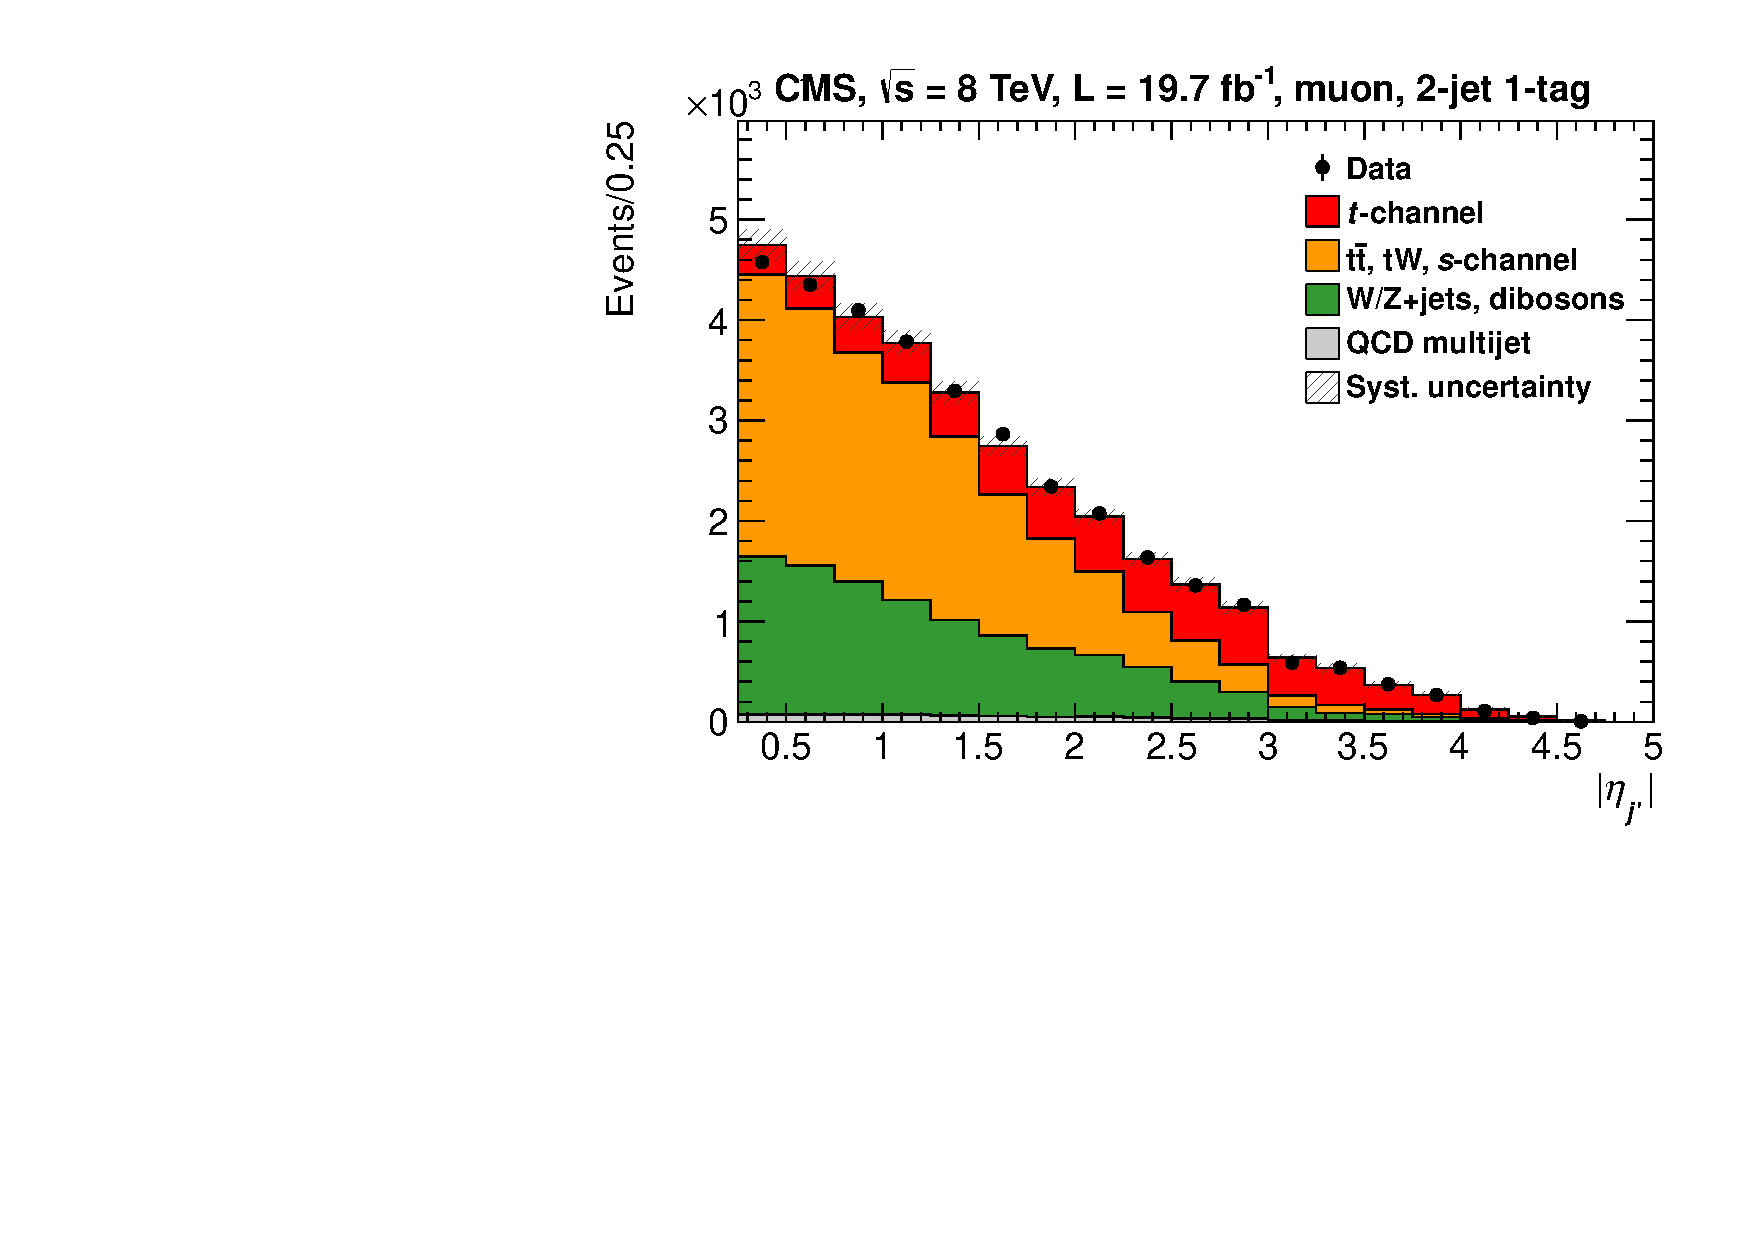
\includegraphics[width=0.46\textwidth]{cms_xsec8/etamuon.pdf}\\(a)}
\parbox[t]{0.42\textwidth}{\centering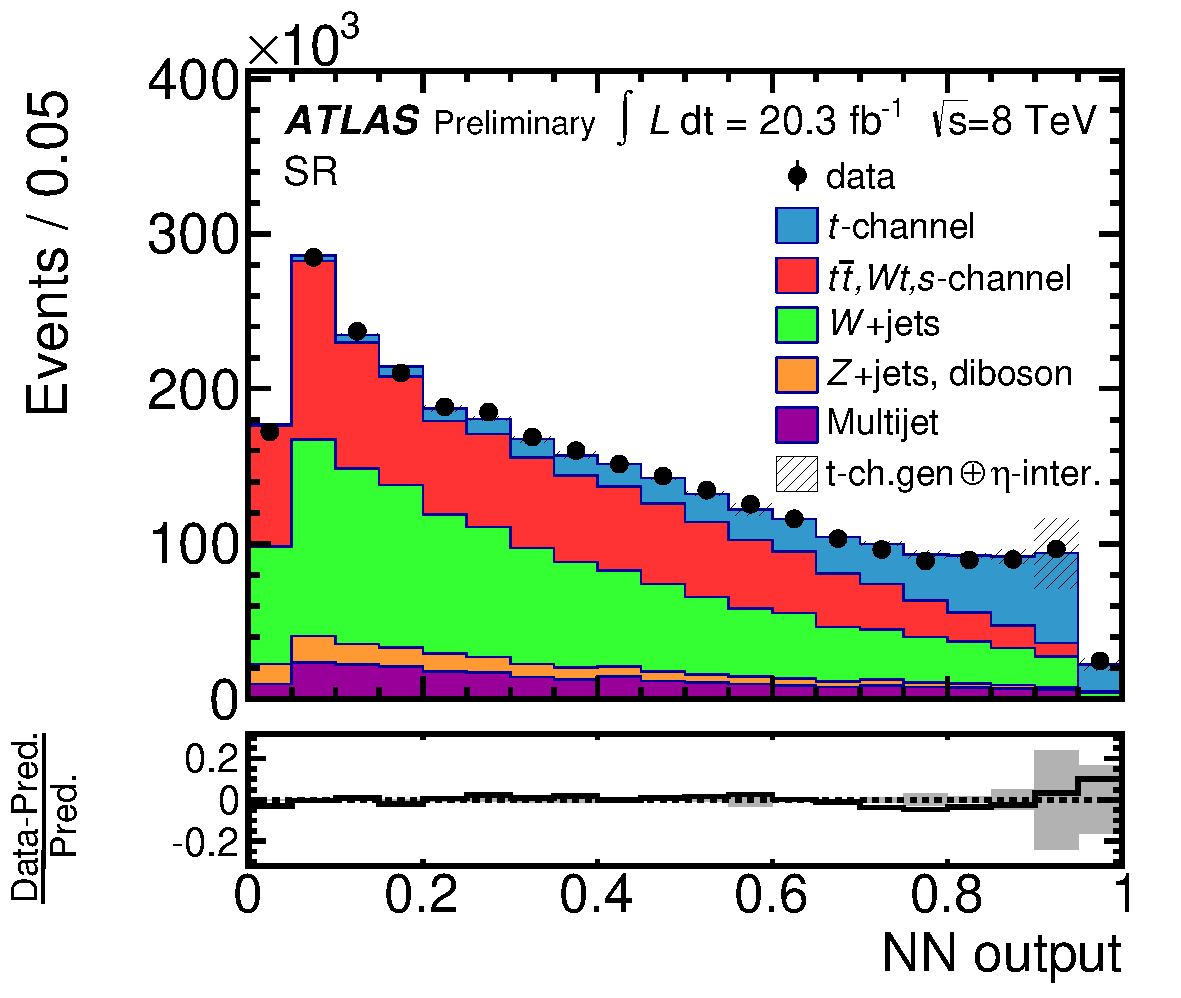
\includegraphics[width=0.37\textwidth]{atlas_xsec8/nnoutput.pdf}\\(b)}

\end{center}
\caption{\label{fig:fit-xsec-8}Discriminating observables used to measure the single top quark cross section: (a)~pseudo rapidity of the non b-tagged jet by CMS and (b)~neutral network output by ATLAS.}

\end{figure}

Finaly, the measured inclusive cross section is used to set a limit on the CKM matrix element $\mathrm{V_{tb}}$ without assumptions on the number of quark generations.

In addition to the inclusive cross section, the fiducial cross section has been measured as well. It provides a deep test of the theory by restricting the measurement only to the detector acceptance. The advantage is that fiducial measurements do not inherit theoretical uncertainities that account for extrapolations into an experimentally unprobed phase space.


The results of the inclusive and fiducial cross section measurements together with the extracted limits on $\mathrm{V_{tb}}$ are summarized in Table ???


\section{Charge ratio measurements}
The cross section charge ratio $\sigma(t)/\sigma(\bar{t})$ has also been measured~\cite{atlas-charge7,cms-xsec8}. It is particular sensitive to the parton distribution functions (PDF). Figure~\ref{fig:charge-ratio} shows measurements by CMS (8~TeV) and ATLAS (7~TeV) compared to different PDF sets. Similar tensions in both measurements for some sets are observed. 

\begin{figure}[htbp]
\begin{center}
\parbox[t]{0.45\textwidth}{\centering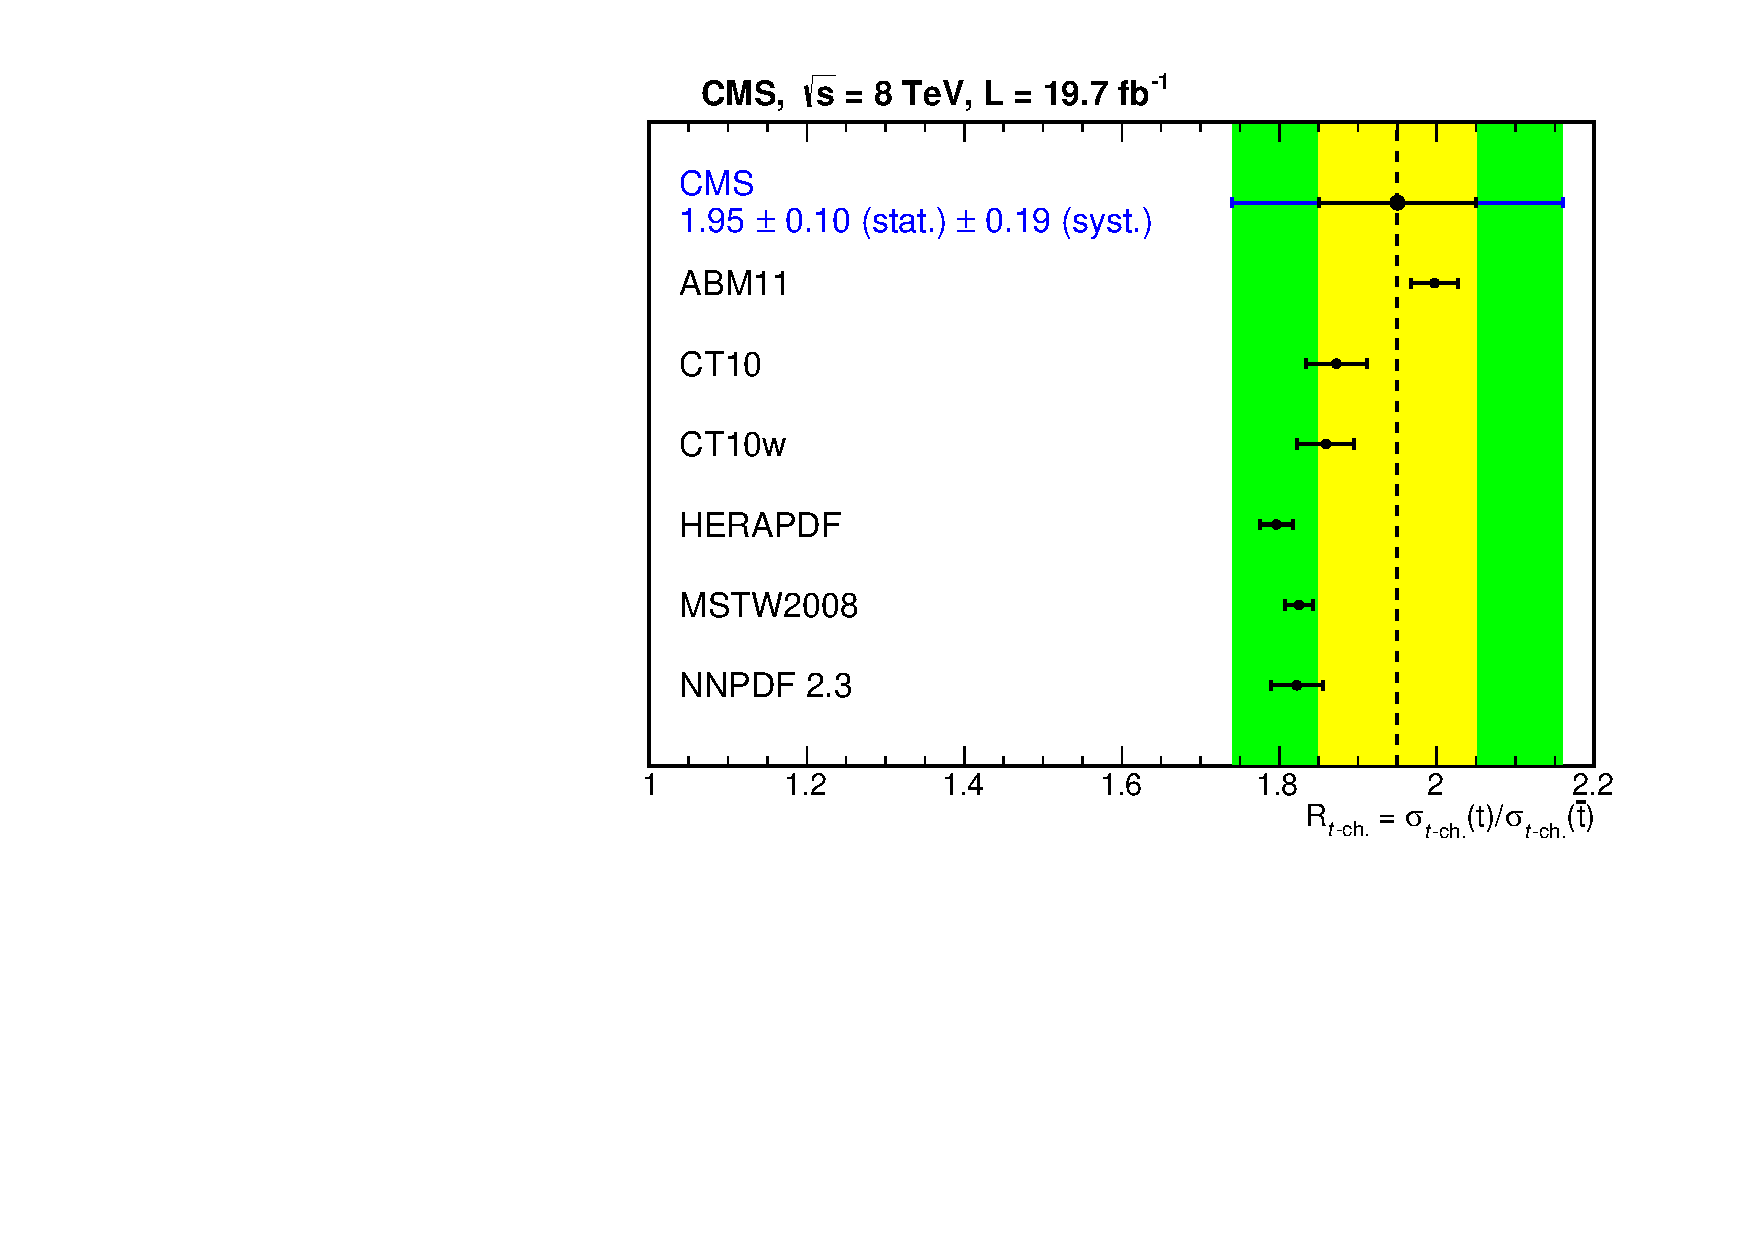
\includegraphics[width=0.4\textwidth]{cms_xsec8/charge.pdf}\\(a)}
\parbox[t]{0.45\textwidth}{\centering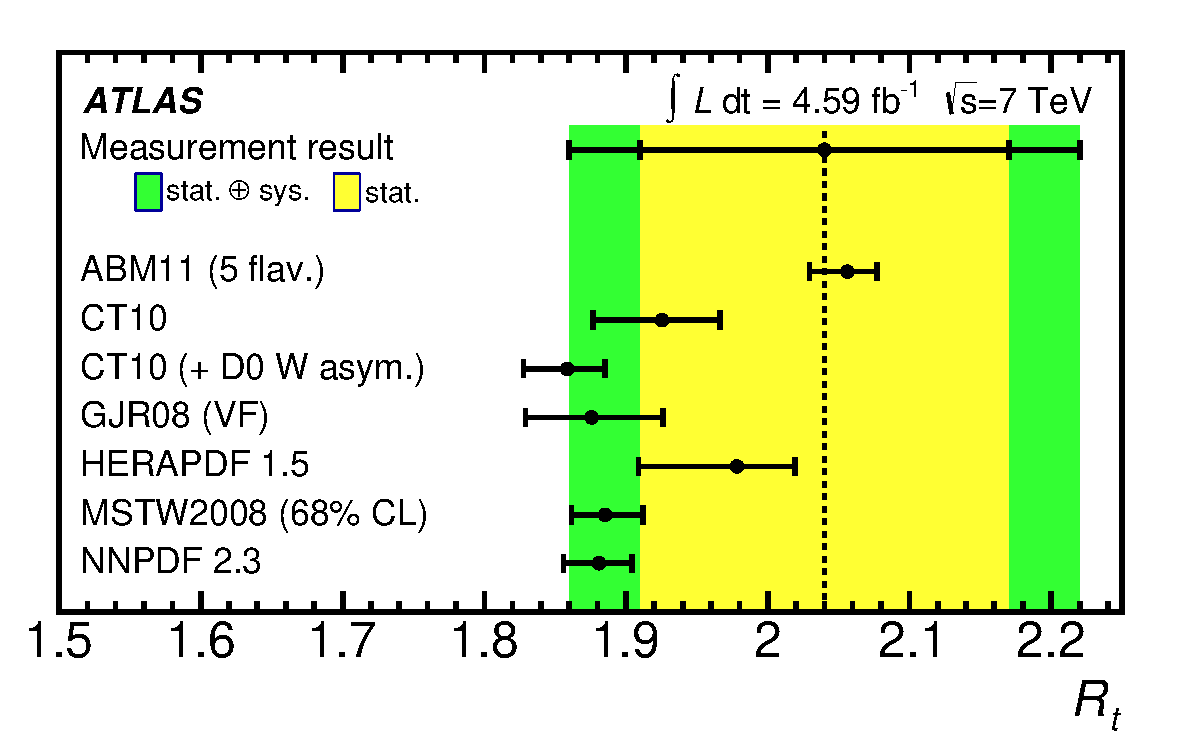
\includegraphics[width=0.4\textwidth]{atlas_charge7/charge.pdf}\\(b)}
\end{center}
\caption{\label{fig:charge-ratio}Charge ratio ???.}

\end{figure}



\section{Properties}

%
\begin{figure}[htbp]
\begin{center}
\parbox[t]{0.3\textwidth}{\centering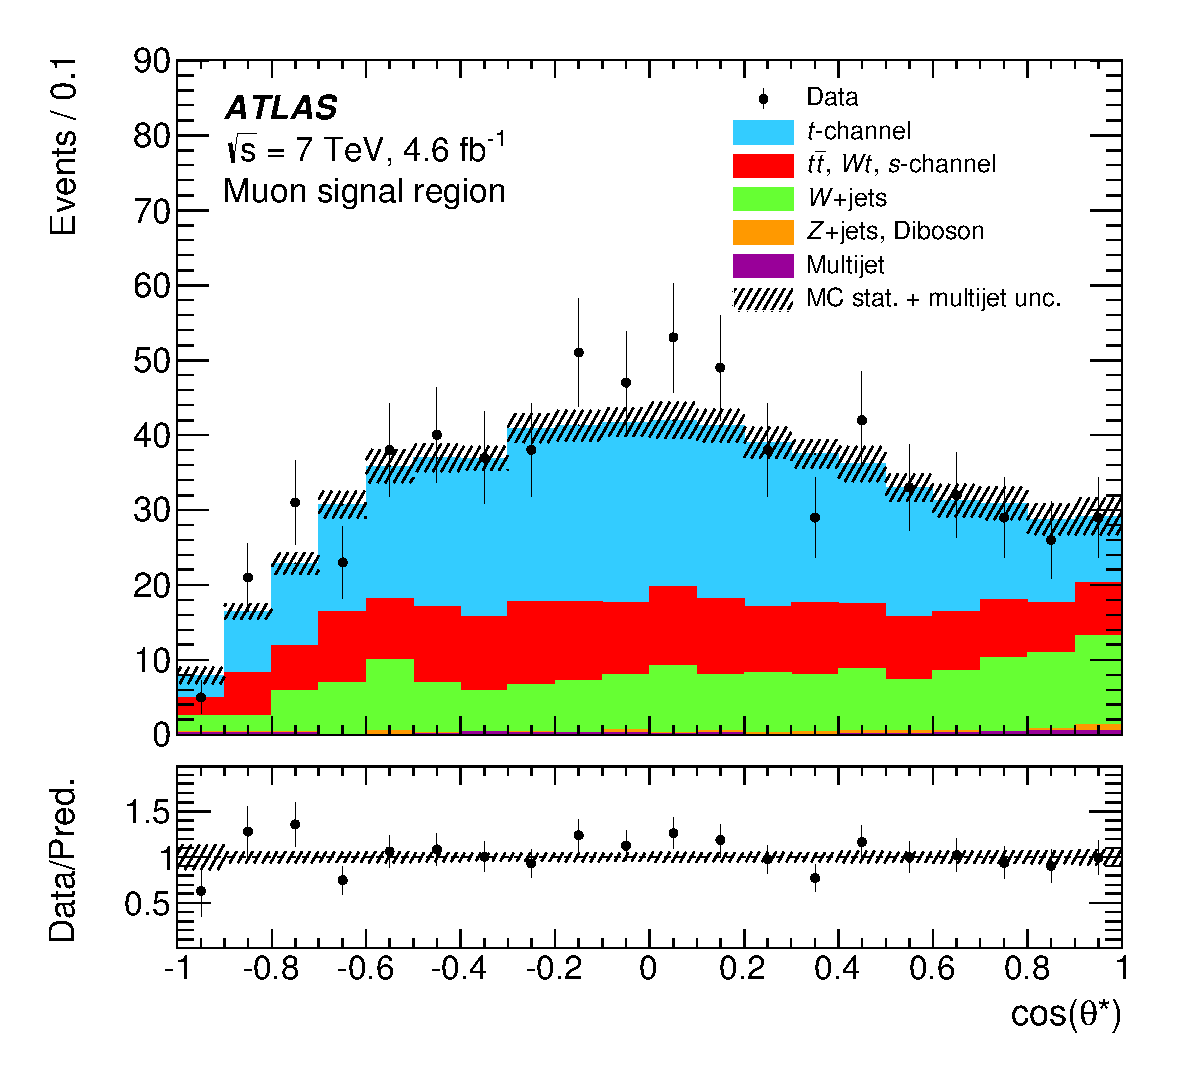
\includegraphics[width=0.29\textwidth]{atlas_anomcoupl/theta.pdf}\\(a)}
\parbox[t]{0.3\textwidth}{\centering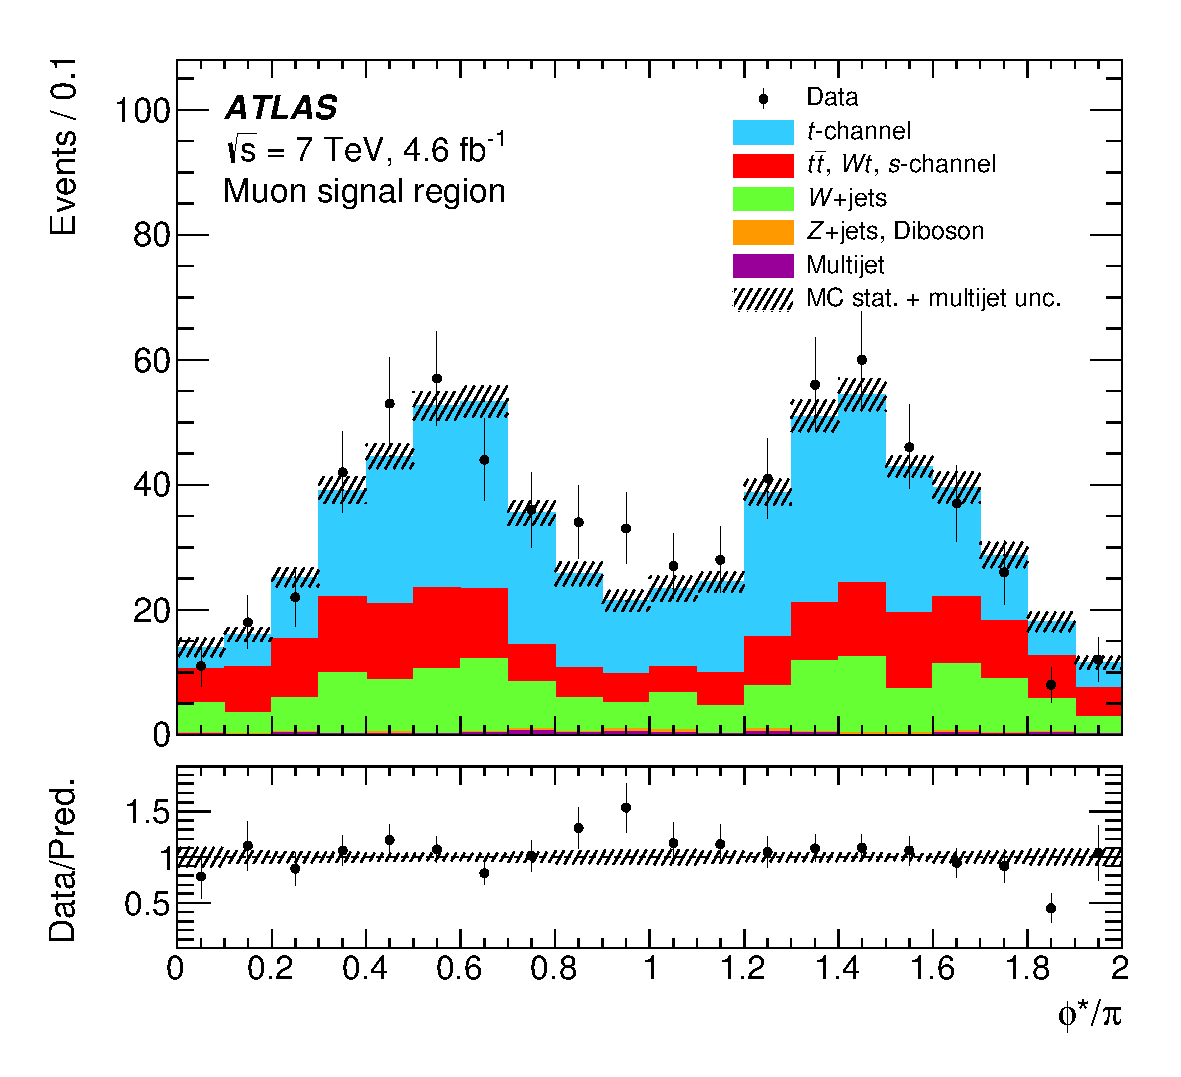
\includegraphics[width=0.29\textwidth]{atlas_anomcoupl/phi.pdf}\\(b)}
\parbox[t]{0.38\textwidth}{\centering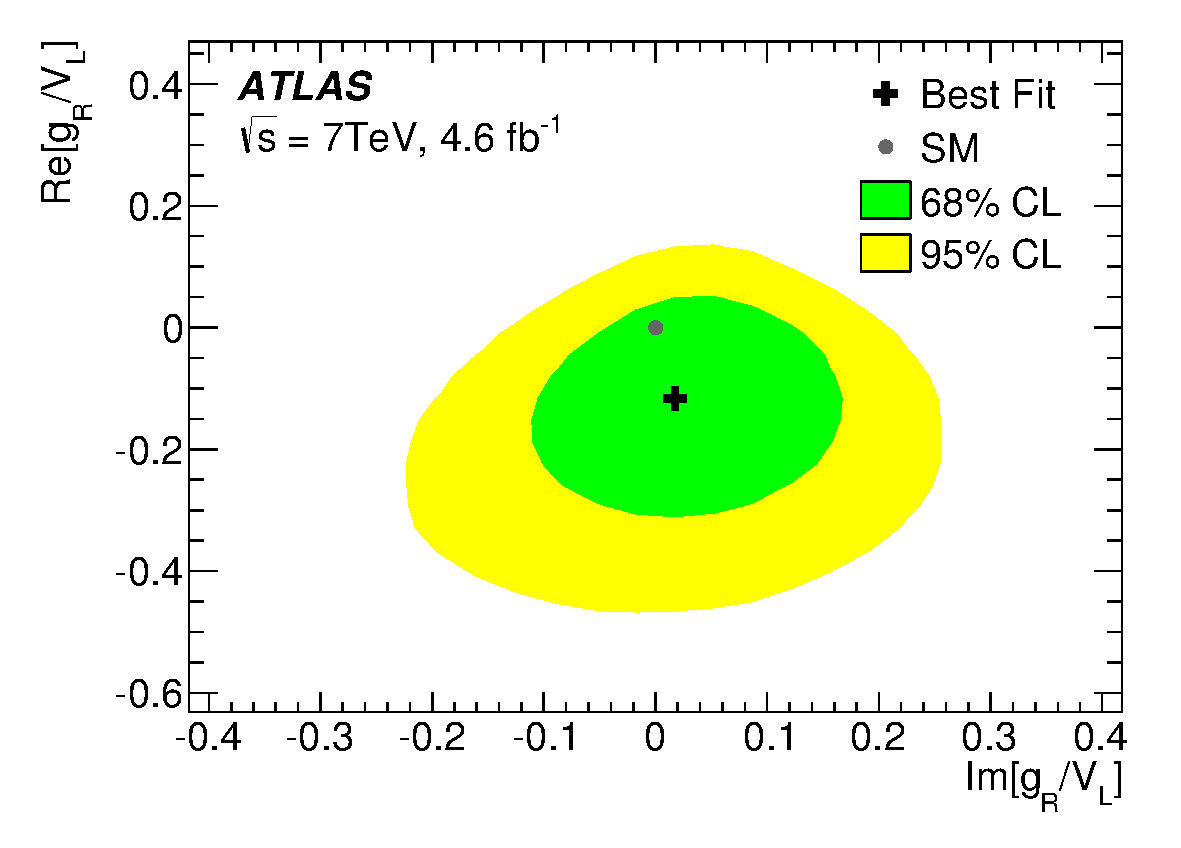
\includegraphics[width=0.36\textwidth]{atlas_anomcoupl/limits.pdf}\\(c)}
\end{center}
\caption{Limits on anomalous couplings~\cite{atlas-anomcoupl}.}
\end{figure}

\section{Early cross section measurement at 13~TeV}

\begin{figure}[htbp]
\begin{center}
\parbox[t]{0.3\textwidth}{\centering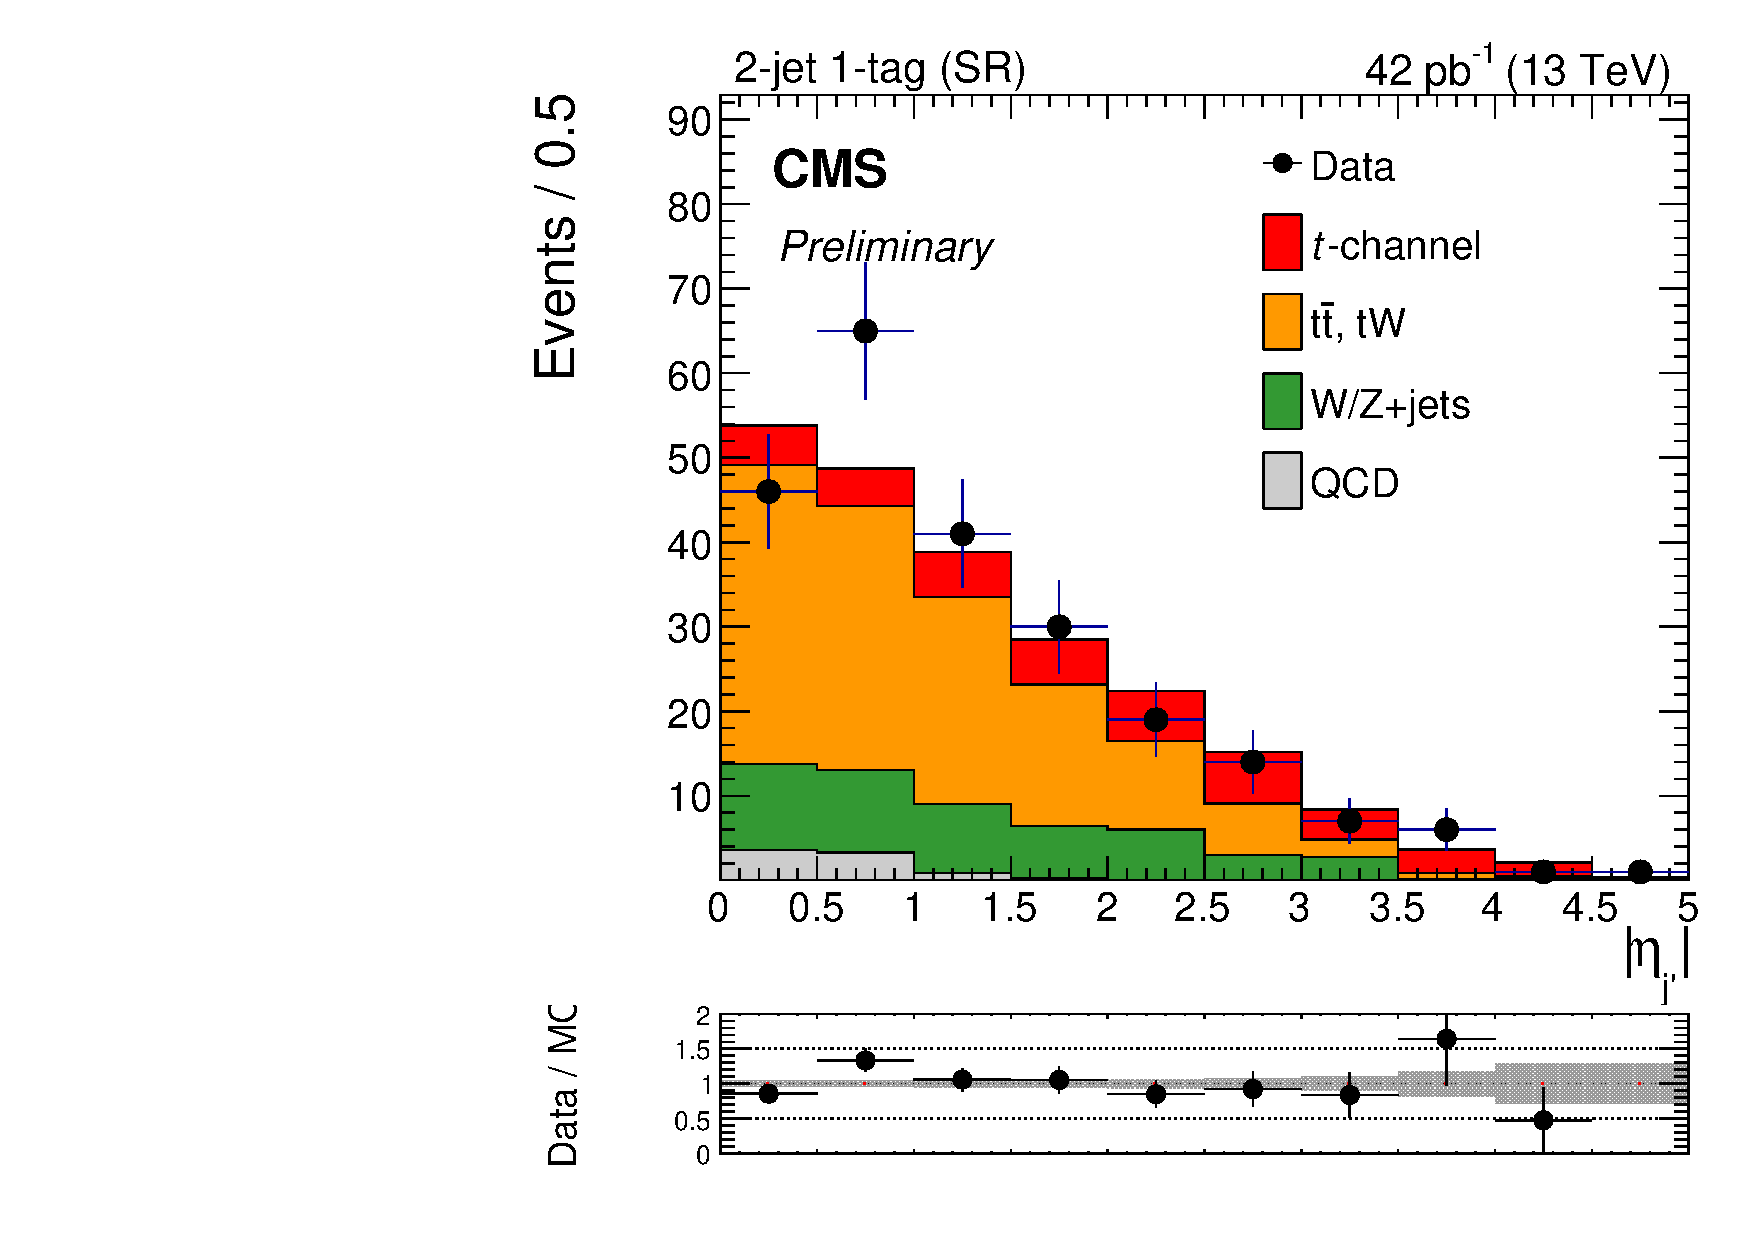
\includegraphics[width=0.28\textwidth]{cms_xsec13/mu2j1t.pdf}\\(a)}
\parbox[t]{0.45\textwidth}{\centering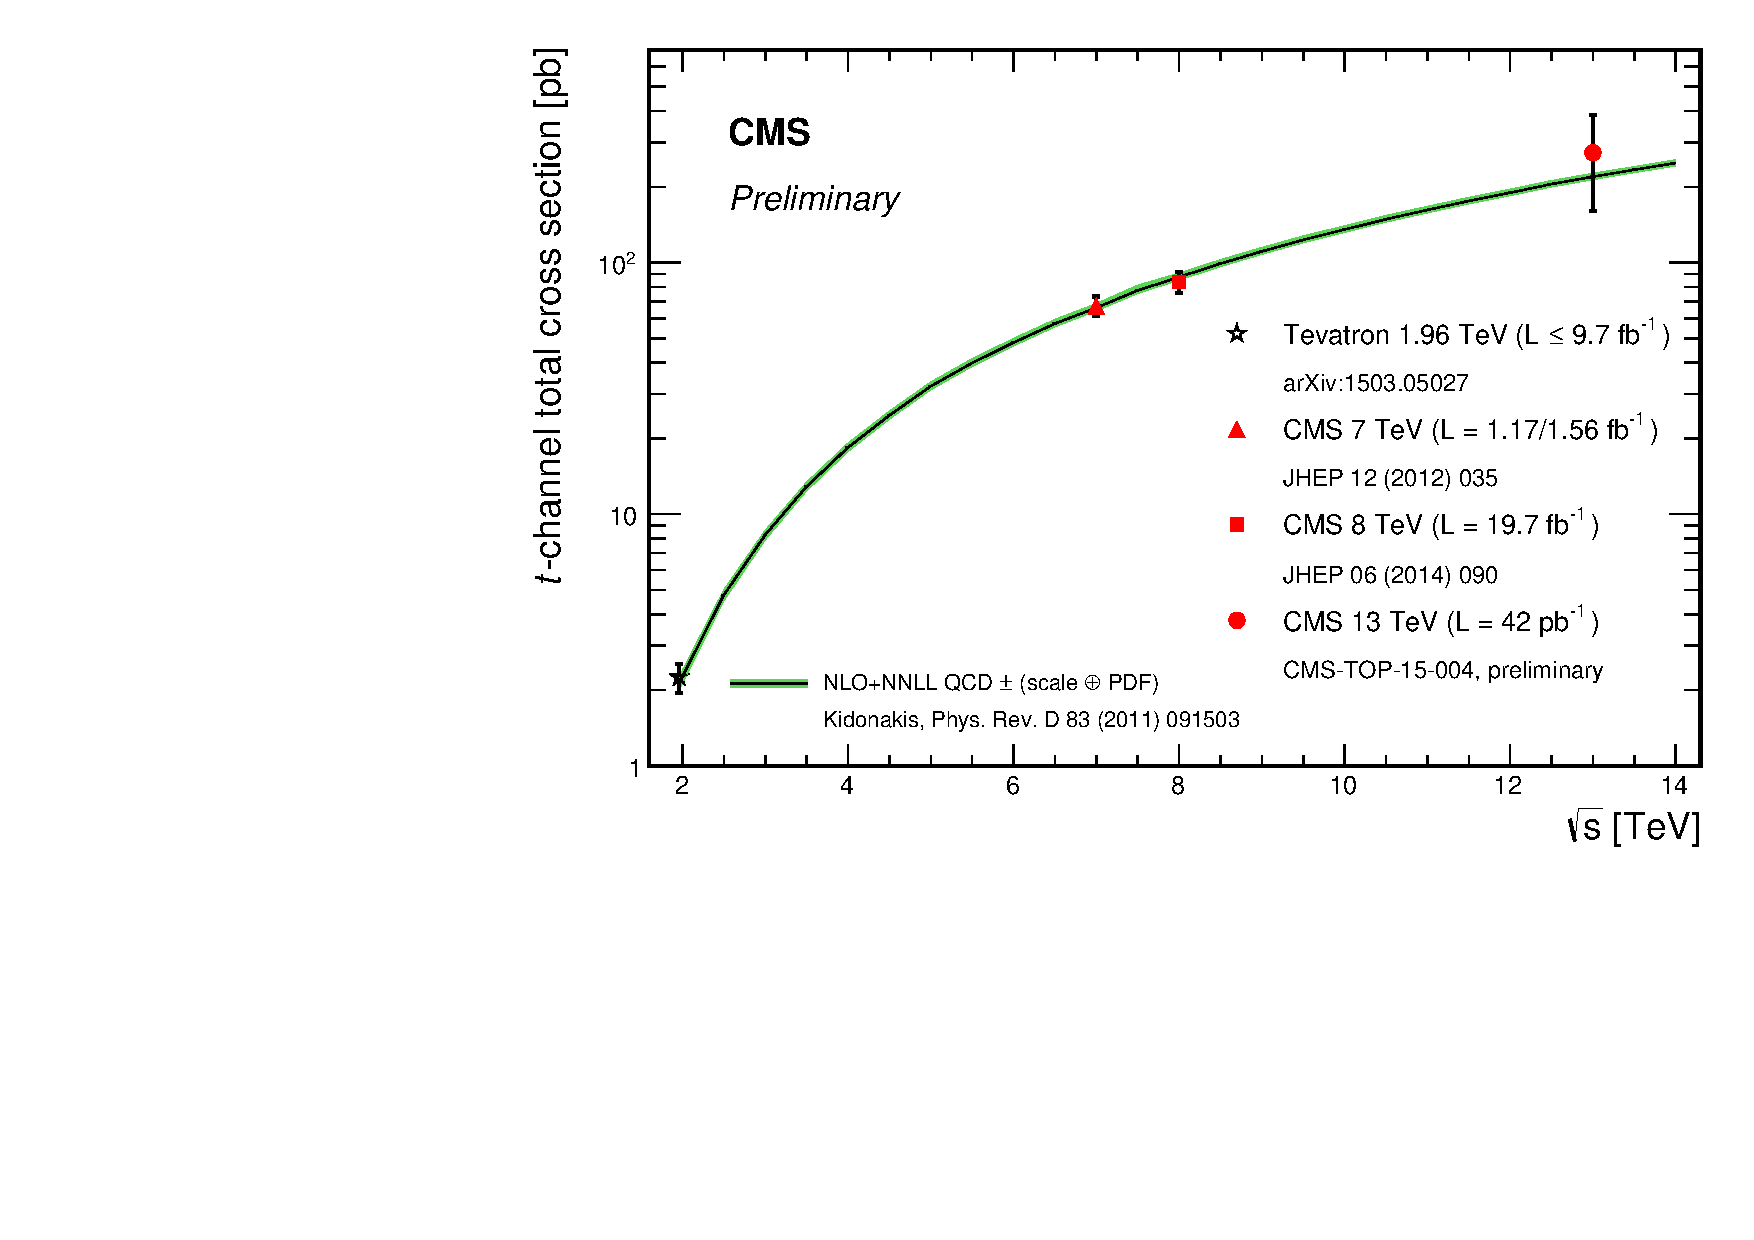
\includegraphics[width=0.4\textwidth]{cms_xsec13/xsec.pdf}\\(b)}
\end{center}
\caption{Measurement of single top cross section at 13~TeV~\cite{CMS-PAS-TOP-15-004}.}
\end{figure}

\section{Conclusion}


\begin{thebibliography}{99}

\bibitem{atlas-anomcoupl}{G. Aad et. al., \emph{Search for anomalous couplings in the $Wtb$ vertex from the measurement of double differential angular decay rates of single top quarks produced in the $t$-channel with the ATLAS detector}, 
\texttt{arXiv:1510.03764[hep-ex]}, 2015.}


\bibitem{atlas-charge7}{G. Aad et. al., \emph{Comprehensive measurements of $t$-channel single top-quark production cross sections at $\sqrt{s} = 7$ TeV with the ATLAS detector}, Phys. Rev. D90 112006, 2014.}

\bibitem{atlas-xsec8}{ATLAS Collaboration, \emph{Measurement of the Inclusive and Fiducial Cross-Section of Single Top-Quark $t$-Channel Events in $pp$ Collisions at $\sqrt{s}$ = 8 TeV}, Tech. Rep. ATLAS-CONF-2014-007, 2014}

\bibitem{cms-xsec8}{V. Khachatryan, et. al., \emph{Measurement of the t-channel single-top-quark production cross section and of the |Vtb| CKM matrix element in pp collisions at $\sqrt{s}$ = 8~TeV}, JHEP06 090, 2014}

\bibitem{CMS-PAS-TOP-15-007}{CMS Collaboration, \emph{Fiducial t-channel single top-quark cross section at 8 TeV}, Tech. Rep. CMS-PAS-TOP-15-007, 2015.}

\bibitem{CMS-PAS-TOP-15-004}{CMS Collaboration, \emph{Measurement of the t-channel single top-quark cross section at 13 TeV}, Tech. Rep. CMS-PAS-TOP-15-004, 2015.}

\end{thebibliography}

\end{document}
